\documentclass[10pt,a4paper,twoside]{book}

% UNICORNS %
\usepackage[british]{babel}
\usepackage{combelow}
\useshorthands{"}
\defineshorthand{"s}{\cb{s}}

% packages
\usepackage{adjustbox}
\usepackage{geometry}
\usepackage{fancyhdr}
\usepackage{url}
\usepackage{amsmath}
\usepackage{amssymb}
\usepackage[algochapter]{algorithm2e}
\usepackage{listings}
\usepackage[usenames, dvipsnames]{color}
%\usepackage{lipsum}
% end packages

\usepackage{color}
\definecolor{lightgray}{rgb}{.9,.9,.9}
\definecolor{darkgray}{rgb}{.4,.4,.4}
\definecolor{purple}{rgb}{0.65, 0.12, 0.82}

\lstdefinelanguage{JavaScript}{
  keywords={typeof, new, true, false, catch, function, return, null, catch, switch, var, if, in, while, do, else, case, break},
  keywordstyle=\color{blue}\bfseries,
  ndkeywords={class, export, boolean, throw, implements, import, this},
  ndkeywordstyle=\color{darkgray}\bfseries,
  identifierstyle=\color{black},
  sensitive=false,
  comment=[l]{//},
  morecomment=[s]{/*}{*/},
  commentstyle=\color{purple}\ttfamily,
  stringstyle=\color{red}\ttfamily,
  morestring=[b]',
  morestring=[b]"
}

\lstset{
   language=JavaScript,
   backgroundcolor=\color{lightgray},
   extendedchars=true,
   basicstyle=\small\ttfamily,
   showstringspaces=false,
   showspaces=false,
   numbers=left,
   numberstyle=\footnotesize,
   numbersep=10pt,
   tabsize=4,
   breaklines=true,
   showtabs=false,
   captionpos=b,
   xleftmargin=0.7cm
}


% configure style of pages

\geometry{a4paper,lmargin=2.5cm,rmargin=2.5cm,tmargin=2.5cm,bmargin=2.5cm}

\renewcommand{\baselinestretch}{1}

\fancypagestyle{plain}{
  \fancyhf{}

  \renewcommand{\headrulewidth}{0.5pt}
  \renewcommand{\footrulewidth}{0.5pt}

  \fancyfoot[C]{\thepage}
}

\fancypagestyle{marked}{
  \fancyhf{}

  \renewcommand{\headrulewidth}{0.5pt}
  \renewcommand{\footrulewidth}{0.5pt}

  \fancyhead[LO]{\slshape \rightmark}
  \fancyhead[RE]{\slshape  \leftmark}

  \fancyfoot[C]{\thepage}
}

\pagestyle{plain}


\begin{document}

% =============================================================================
% Title page

 \newpage
  \thispagestyle{empty}

    \adjustbox{padding={5pt},frame={1pt},right}{Dissertation Type: research}

  \vspace*{\fill}
  \begin{center}
                
\includegraphics[scale=0.3]{logo/logo_uob_color}                \\
                              \vspace*{1.0cm}
                          DEPARTMENT OF COMPUTER SCIENCE                        \\
                              \vspace*{2.0cm}
                       
 				 \mbox{{\LARGE Timing Attacks in the Modern Web}} \\
                              \vspace*{0.5cm}
                              \vspace*{1.0cm}
                          {\Large Ana-Maria Dumitra"s}                         \\

                              \vspace*{1.0cm}
                          \rule{0.5\textwidth}{0.5pt}
                              \vspace*{1.0cm}

            A dissertation submitted to the University of Bristol
            in accordance with the requirements of the degree of
            Master   of Engineering
                    in the Faculty of Engineering.                                

                              \vspace*{1.0cm}
                          \rule{0.5\textwidth}{0.5pt}
                              \vspace*{1.0cm}

                                  \today
  \end{center}
  \vspace*{\fill}
  
%==============================================================================
% Front matter

\cleardoublepage
\pagestyle{plain}
\pagenumbering{roman}

% =============================================================================
% Declaration

\newpage
  \thispagestyle{plain}

  \chapter*{Declaration}

  This dissertation is submitted to the University of Bristol in accordance 
  with the requirements of the degree of MEng in the Faculty 
  of Engineering.  It has not been submitted for any other degree or diploma 
  of any examining body.  Except where specifically acknowledged, it is all 
  the work of the Author. 

  \vspace{6cm}

  \noindent {Ana-Maria Dumitra"s}, \today


\tableofcontents
\listoffigures
%\listoftables
\listofalgorithms
\lstlistoflistings

%========================================================================================================

% -----------------------------------------------------------------------------


\chapter*{Executive Summary}

% -----------------------------------------------------------------------------

\chapter*{Supporting Technologies}

\begin{quote}
\noindent
\begin{itemize}
\item HTML
\item CSS
\item JavaScript
\item AngularJS 1
\item Bootstrap
\item jQuery
\item Google Chart Angular
\item mathjs
\item NodeJS
\item Magic ...
\end{itemize}
\end{quote}

% -----------------------------------------------------------------------------

\chapter*{Notation and Acronyms}

% {\bf An optional section, of roughly $1$ or $2$ pages}
% \vspace{1cm} 

% \noindent
% Any well written document will introduce notation and acronyms before
% their use, {\em even if} they are standard in some way: this ensures 
% any reader can understand the resulting self-contained content.  

% Said introduction can exist within the dissertation itself, wherever 
% that is appropriate.  For an acronym, this is typically achieved at 
% the first point of use via ``Advanced Encryption Standard (AES)'' or 
% similar, noting the capitalisation of relevant letters.  However, it 
% can be useful to include an additional, dedicated list at the start 
% of the dissertation; the advantage of doing so is that you cannot 
% mistakenly use an acronym before defining it.  A limited example is 
% as follows:

\begin{quote}
\noindent
\begin{tabular}{lcl}
% AES                 &:     & Advanced Encryption Standard                                         \\
% DES                 &:     & Data Encryption Standard                                             \\
%                     &\vdots&                                                                      \\
% ${\mathcal H}( x )$ &:     & the Hamming weight of $x$                                            \\
% ${\mathbb  F}_q$    &:     & a finite field with $q$ elements                                     \\
% $x_i$               &:     & the $i$-th bit of some binary sequence $x$, st. $x_i \in \{ 0, 1 \}$ \\

AES			   	 	&:	   & Advanced Encryption Standard							 \\	
AppCache		   	 	&:	   & Application Cache   									 \\	
CPU					&:	   & Central Processing Unit									 \\
CSS					&:	   & Cascading Style Sheets									 \\
DES					&:	   & Data Encryption Standard								 \\
DRAM					&:	   & Dynamic Random Access Memory							 \\
HTML					&:     & HyperText Markup Language								 \\
RAM					&:	   & Random Access Memory									 \\
RSA					&:	   & Rivest-Shamir-Adleman Cryptosystem				    		 \\
SCA					&:	   & Side-Channel Attack										 \\	
SRAM					&:	   & Static Random Access Memory								 \\
\end{tabular}
\end{quote}

% -----------------------------------------------------------------------------

\chapter*{Acknowledgements}

\noindent
%I would like to thank Clifton Suspension Bridge, Sergey Brin and gin.


%========================================================================================================
% Main matter
\cleardoublepage
\pagestyle{marked}
\pagenumbering{arabic}
\parindent=0in
\parskip=1em 

%%%%%%%%%%%%%%%%%%%%%%%%%%%%%%%%%%%%%%%%%%%%%%%%%%%%%%%%%%%%%%%%%%%%%%%%%%%%%%%%%%%%%%%%%%%%%%%%%%%%%%%%%
%%%%%%%%%%%%%%%%%%%%%%%%%%%%%%%%%%%%%%%%%%%%%% UNICORNS %%%%%%%%%%%%%%%%%%%%%%%%%%%%%%%%%%%%%%%%%%%%%%%%%
%%%%%%%%%%%%%%%%%%%%%%%%%%%%%%%%%%%%%%%%%%%%%%%%%%%%%%%%%%%%%%%%%%%%%%%%%%%%%%%%%%%%%%%%%%%%%%%%%%%%%%%%%

% -----------------------------------------------------------------------------

\chapter{Contextual Background}
\label{chap:context}


% -----------------------------------------------------------------------------

\chapter{Technical Background}
\label{chap:technical}

%%%%%%%%%%%%%%%%%%%%%%%%%%%%%%%%%%%%%%%%%%%%%%%%%%%
%%%%%%%%%%%%%%%%% Vampires %%%%%%%%%%%%%%%%%%%%%%%%
%%%%%%%%%%%%%%%%%%%%%%%%%%%%%%%%%%%%%%%%%%%%%%%%%%%

\section{Side-Channel Attacks}

Timing information, power consumption, electromagnetic emission or heat dissipation measured while the device performs an interesting operation can reveal sensitive information. These leaks based on physical characteristics are known as \textit{Side Channels}. Side-Channel Attacks (SCA) are a powerful set of attacks which rely on recovering secret data by analysing the device rather than exploiting vulnerabilities in the underlying algorithm. 

The idea of using Side-Channel information to attack cryptographic schemes was introduced by Kocher in his 1996 paper \cite{kocher1996timing}. Kocher proved that it is possible to find fixed Diffie-Hellman exponents, factor RSA keys and break other cryptosystems by analysing the time it takes to perform certain operations. Side-Channel Attacks try to find the correlation between the side channel information and the internal state of the processing device which is related to the secret parameters involved in the computation. 

The literature classifies physical attacks by either the level of intrusion (invasive or non-invasive attacks) or the degree of interaction between the adversary and the victim (passive or active attacks).
\begin{enumerate}
\item Invasive \textit{vs.} non-invasive: Invasive attacks refer to techniques where the device under attack is permanently modified in order to capture information stored in memory areas or data flowing through the data bus, registers, etc.\cite{Tria2011}. Non-invasive attacks only use externally available information such as running time, power consumption, electromagnetic emission or heat emission \cite{standaert2010introduction}.
\item Active \textit{vs.} passive: Active attacks require the adversary to tamper with the device by either causing the algorithm to execute incorrectly (\textit{Fault Injection}) or modifying any part of the physical implementation. In contrast, a Passive Attack or Side-Channel Analysis will monitor the device's behaviour and record variations of the execution time (\textit{Timing Attack}), the power consumption (\textit{Power Analysis}), the electromagnetic emission (\textit{Electro-magnetic analysis - EMA}) or the state of the cache memory (\textit{Cache Attacks}).
\end{enumerate}

Side-Channel Attacks are an important class of cryptanalytic techniques. In general, cryptanalysis focuses on studying systems in order to uncover weaknesses that might lead to finding the secret information. Side-Channel Attacks target a specific implementation rather than an abstract algorithm, making them less generic but more powerful \cite{standaert2010introduction}.

\subsection{Timing Attacks}

Timing attacks are one of the oldest categories of side channel attacks, where time measurements are used to recover the secret information. The basic idea behind timing attacks is to learn the secret key based on how long it takes to perform certain operations. In older systems, the time varied depending on the data and the cryptographic key, which would allow an attacker to easily learn the secret information \cite{Koeune2011}.

The first side-channel attack using timing information was discovered by Kocher in \cite{kocher1996timing}, where he describes how to break various cryptosystems. Kocher was able to obtain the secret key due to faults in the algorithm's implementations which leaked information about the private data.

For example, RSA \cite{rivest1978method} requires the computation of $m = c^d \, mod \, N$, where $N$ is the public key and $c$ can be found by an adversary. The attacker's goal is to find the value of $d$. The attack uses the fact that for every bit set in the private key $d$, the time to execute the modular exponentiation increases. Therefore, an attacker after computing the modular exponentiation for several values of $c$, could determine the secret value $d$ \cite{kocher1996timing}.

\subsection{Cache Attacks}
Cache attacks are a particular kind of Side-Channel Attacks, which monitor how processes currently running on the device alter the cache memory. Cache attacks are not affected by higher-level security mechanisms, like protection rings, virtual memory, hypervisors and sandboxing. Cache attack are easy to run as they do not require special equipment or excessive computational power. The only requirement is that the attacker is able to run a spy program which shares the cache memory with the victim \cite{oren2015spy}.

If timing attacks exploit vulnerabilities in the cryptographic algorithm's implementation that could lead to the discovery of the secret key, cache attacks target the actual device and make use of the fact that memory access is not always performed in constant time \cite{canteaut2006understanding}.

The idea of using cache memory as a side-channel was first proposed by Hu in \cite{hu1992lattice}. He was the first to suggest that the time difference between a cache hit and a cache miss can be used to learn more about the internal state of the system. In 1998 Kelsey et al. proposed that this information be used to attack cryptographic systems in \cite{kelsey1998side}. 

Despite cache vulnerabilities being known for some time, actual cache attack have not been developed until early 2000s. The idea proposed by Kelsey et al. was later expanded by Page in \cite{page2002theoretical}, who described a theoretical attack against DES. A year later, Tsunoo et al. demonstrated a cache attack against DES and proposed a similar attack against AES \cite{tsunoo2003cryptanalysis}.

In 2006, Osvik et al. presented a cache attack against AES based on inter-process leakage \cite{osvik2006cache}. Their paper also describes the PRIME+PROBE algorithm in the context of the first level cache, L1, which was later extended to last level cache (LLC) by Liu et al. \cite{liu2015last}. Oren et al. proposed a new category of cache attacks which affect browsers. Their attack builds on the work of Liu et al. and uses information about the cache memory to determine a user's browsing activity \cite{oren2015spy}.

\subsection{Browser Attacks}
Traditionally, web browsers were software applications which allow users to view and interact with content on a web page. The expansion of the Internet determined browser vendors to add new features to their software. The transition from static to dynamic web pages, not only brought richer, more interactive and responsive web applications but also opened the way for a new series of attacks, known as browser attacks. The most popular attacks amongst web applications are by far cross-site scripting (XSS) and SQL injection, over the last few years there has been an increase in attacks of web applications targeting side channel information such as the time it takes to load an external resource.

One of the most popular browser attacks is the disclosure of pages the user has previously visited. The majority of browsers change the color of a link if the user has visited it before. The change can easily be done by using the CSS:visited pseudo-class. An attacker can request the computed style using JavaScript and therefore gaining access to the victim’s browsers history \cite{cssvisited}. Researchers discovered that this techniques was being used by numerous high-profile websites to obtain a user’s browsing history
\cite{jang2010empirical}.

Analysing the style of a web page is not the only way to expose a user’s browsing history. A similar attack discovered by Felten et al. \cite{felten2000timing} uses timing information to determine if a web page has been previously visited by the victim. This attack assumes that recently accessed resources will be cached by the browser in order to provide faster loading times for future visits. By comparing the loading time of different web pages an attacker can determine if a file is in the user’s cache, and hence whether or not the user has accessed the file before.

Websites customize their services according to users’ locations. For example a user accessing Google from within the United Kingdom will be redirected to www.google.co.uk. Jia et al. have shown that is possible to derive a user’s location by simply checking what version of the website they are redirected to \cite{jia2015know}.

Another class of browser attacks was identified by Bortz et al. in \cite{bortz2007exposing}. If previous attack were targeting static resources, which can be caches, their attack is aimed at dynamically generated web pages. Bortz et al. present two types of attacks: \textit{direct timing} attacks, where an adversary has direct access to a website and is able to obtain information about the website's state by simply measuring the server's response time, and \textit{cross-site timing} attacks, where an adversary tries to obtain information about the victim's view of a cross-origin website.

The measurements techniques used by Bortz et al. were dependent on network conditions and could provide erroneous results. Van Goethem et al. extended their work and presented new timing methods which are independent of the victim's network condition, thus provide more accurate timing information in \cite{van2015clock}. 

Oren et al. identified a new category of side-channel attack which run in the browser. They used JavaScript to spy in a remote user's browsing activity. The work described in \cite{oren2015spy} uses the state of the browser's cache memory to determine what web site the victim is currently visiting.
\section{Cache Memory}

Cache memory is a small high-speed memory, usually SRAM, located inside the CPU chip. The main role of the cache memory is to speed up the overall runtime of the system by providing fast access to frequently used resources. Cache memory acts as a buffer between the high speed CPU and the slower main memory or DRAM.

A system can only be as fast as its slowest component. Early computers had extremely slow main memory, but CPU were not fast either and their speed was increasing at roughly the same rate. Starting in the 1980s, the CPU clock speed started to increase while memory access time remained relatively slow. Despite having faster CPUs, machines were still slow due to the memory access bottleneck. The increasing gap between CPU speed and memory access time led to the development of the first CPU caches. Nowadays, cache memory is included in every modern CPU from the ultra-low power chips to the highest-end Intel Core i7.

Cache memory increases the overall speed of the system by granting fast access to frequently accessed main memory contents. The algorithm which decides what resources to be stored in cache varies from one architecture to another and is known to change between processor generations \cite{oren2015spy}. 

The structure of the cache memory follows a hierarchical scheme. The top level contains the level 1 (L1) cache which is the smallest, fastest and closest to the CPU. The L1 cache is followed by a series of progressively larger and slower memory elements until it reaches the main memory. Typically the cache is split into three levels: L1, L2 and L3. The cache level closest to the RAM is known as last-level cache or LLC \cite{oren2015spy}.

Multi-level caches split into two categories: inclusive and exclusive cache. Inclusive cache requires that lower levels of the cache include all the data which can be found in the upper levels. Exclusive caches guarantee that data can be found in at most one cache level. The two designs have various advantages and disadvantages. Exclusive caches allow more data to be stored while removing data from inclusive caches is generally faster since it only needs to be removed from the last-level cache. Intel's cache architecture is inclusive while AMD's cache architecture is exclusive \cite{oren2015spy}.

When the CPU need to access physical memory it will first look for the respective address in the cache. If the resource does not reside in the cache memory, it will have to be retrieved from the main memory. This is known as a \textit{Cache miss}. A \textit{Cache hit} occurs when the address the CPU is looking for is found in any of the cache memory levels \cite{oren2015spy}.

% cite an overview of cache by intel
% http://download.intel.com/design/intarch/papers/cache6.pdf
\subsection{Cache Organization}
Since cache memory is generally smaller than main memory, various techniques are used to map main memory to cache. Main memory is split into cache pages, a cache page is a block of main memory which size is dependent on the cache memory. Each cache page is further divided into cache lines. Based on the mapping mode caches can be split into: direct mapped, n-way set associative and fully associative cache.
\begin{itemize}
\item Direct Mapped: Direct Mapped Cache is also known as 1-way set associative cache. In direct mapped mode, the main memory is divided into cache pages equal to the size of the cache. Each cache line can only reside in one position in the cache memory. 
\item Fully Associative: Fully Associative Cache allows any cache line from the main memory to reside anywhere in the cache memory. In a fully associative scheme, the main memory is only divided into cache lines and pages are completely ignored.
\item N-way Set Associative Cache: A Set Associative Cache scheme is a combination of the previous two schemes and the most common technique to map CPU caches. The cache memory is split into n equal blocks known as cache ways. The main memory is split into cache pages of size equal to the cache way. Each cache way acts like a small direct mapped cache. Each cache line can now be stored in n positions in the cache memory. This decreased the need to overwrite the data in the cache memory.
\end{itemize}

\subsection{Intel's Last-Level Cache Structure}
Intel's cache architecture is inclusive, so the last level cache contains all the elements stored in the cache. The LLC is divided into slices one for each core of the CPU. Each core is directly connected to a cache slice but also has access to all the other slices \cite{oren2015spy}.

The size of the LLC varies between processor models and ranges between 3MiB and over 20MiB. Due to its relatively large size it is not efficient to iterate through the whole cache when looking for a specific address. The LLC is further divided into cache sets, each block of main memory maps to a specific set in the cache memory. Each cache set contains several cache lines \cite{oren2015spy}. 

The Intel Core i7-4960HQ processor is multi-core 4th generation Intel Core processor. The cache memory for this processor has a Smart Cache architecture. Smart Cache is an architecture developed by Intel that allows multi-core processors to share the same last level cache memory instead of having dedicated per-core cache. The processor has 8192 ($2^{13}$) cache sets, each set being 12-way associative. Every cache set can hold 12 lines of  64 ($2^6$) bytes each. The total cache size of the Intel Core i7-4960HQ processor is 8192x12x64=6MB \cite{oren2015spy}.

Each cache line can only be stored in 12 positions in the cache memory. The algorithm that determines the mapping between a physical address and an index in cache memory is not public and has changed between processor generations \cite{oren2015spy}. Hund et el. \cite{hund2013practical} were able to reverse engineer the mapping in the case of Sandy Bridge processors.

\section{Web Browsers}

A web browser is a software used for interacting with web applications. The main functions of web browsers are retrieving the requested resource and displaying it in the browser window. In order to display the web document, browsers use rendering engines. There are multiple rendering engines available and different browsers use different engines. According to \cite{statcounter} the top 3 most popular browsers among desktop and tablet users are Chrome (56\%), Firefox(14\%) and Internet Explorer(12\%). They all use different rendering engines, Chrome uses Blink, Firefox uses Gecko while IE uses Trident\cite{howbrowserswork}.

Rendering engines parse the HTML documents and create an output tree made out of DOM, Document Object Model, nodes. The rendering engine is also responsible for gathering all the style information about the DOM nodes. The final output of the engine is the render tree which is ready to be displayed by the browser\cite{howbrowserswork}.

The DOM is a programming interface which allows a more versatile way of accessing the HTML document. It can be easily manipulated by scripting or programming languages in order to change the structure, style or content of the original document\cite{dom}.

\section{HTML}
HyperText Markup Language, known as HTML, is a markup language used to create web pages. Initially designed as a language for semantically describing scientific documents, HTML became the standard markup language for building web documents. HTML is used to describe the structure and semantic content of a web page but not its functionality\cite{world1999html}.

HTML consists of a set of elements, which define the structure of web pages. Most HTML elements are composed of a start tag, \texttt{<element>}, and an end tag, \texttt{</element>} ,with the content nested in between the two tags. The end tag is optional and all browsers will display documents which do not contain a matching closing tag for each opened tag; however this technique can produce unexpected results and it is not recommended. Furthermore, strict HTML document validators require that elements have both a start and an end tag\cite{world1999html}.

HTML also includes a number of empty elements, elements formed of only a start tag or a start tag with the backslash appended to the element name, \texttt{<element/>}, with no content, such as \texttt{<br>}, which defines a line break. The HTML standard does not specify which of the two ways of representing an empty element is preferred. Though, the latter provides stricter validation and is accepted by XML parsers\cite{world1999html}.

HTML elements can have attributes. Attributes are key, value pairs which determine the behaviour of elements, such as \texttt{color}, \texttt{font} or \texttt{position}. Attributes must be specified in the element's start tag\cite{world1999html}.

% sentence about why we need html 5, need of standards something else ?
HTML5 is the 5th version and the current version of the HTML standard. It was released in 2014 by the World Wide Web Consortium (W3C). The current version of HTML introduced a number of new features aimed at simplifying the incorporation of multimedia and graphical content into web based applications\cite{berjon2014html}.

\subsection{Media Elements}
HTML elements are the basic building blocks of web pages. Apart from providing the overall structure of the web page, some HTML elements are used to embed media into a web page. HTML has always provided support for embedding media into web pages, newer versions of the language further simplify the process by introducing elements aimed exactly at this. The \texttt{<img>} element, available sine HTML 4.1, allows the insertion of images while the \texttt{<audio>} and \texttt{<video>} elements introduced in HTML5 enable audio and video content incorporation into web applications.

\subsubsection{Image}
The \texttt{<img>} tag is used to represent an image in a HTML document. The address to the resource to be displayed is stored in the \texttt{src} attribute. In order to successfully embed an image in a web page, the \texttt{src} attribute must be present and it must contain a valid non-empty URL\cite{berjon2014html}.

The browser starts by downloading the external resource from the address provided in the \texttt{src} attribute or an alternative address if this is not available. The \texttt{load} event is delayed until the image data has been fetched over the network. Once the image file has finished downloading, the browser will try to display it. If the value of the \texttt{src} attribute does not link to a valid image file, the \texttt{error} event will be triggered on the \texttt{Image} element\cite{berjon2014html}.

\subsubsection{Video and Audio}
The \texttt{<video>} and \texttt{<audio>} elements were introduced in HTML5 and enable web developers to easily embed audio and video content into their applications. The most recent version of HTML makes the insertion of a video into a web application as easy as adding an image \cite{berjon2014html}.

Similarly to the \texttt{<img>} element, the \texttt{Video} and  \texttt{Audio} elements will first download the external resource and then try to play it. However, these new media elements will not throw an error unless they have finished parsing the entire file\cite{berjon2014html}.

In order to display a media file, the browser will start by downloading the external resource. While the file is being downloaded the \texttt{progress} event is being triggered. When the file has been fetched or if the downloading process has been paused the \texttt{suspend} event is fired. The browser proceeds by parsing the contents of the file to obtain information such as the length, width, height or extension, etc. of the file. If the media resource is not a valid file the browser will not be able to display it and the \texttt{error} event will be triggered on the media element. The time elapsed between the \texttt{suspend} and the \texttt{error} events is depended on the size of the file. The \texttt{error} event fires on the media element when the browser has finished parsing the file in contrast to the \texttt{Image} element, where the event is triggered when the browser learns that the file is not valid, usually as soon as it starts parsing it\cite{berjon2014html}.

\section{JavaScript}
JavaScript is an interpreted scripting language generally used on the client side of web applications. Developed independently by both Netscape and Microsoft, it has been standardized by ECMA International under the name ECMAScript.
The most recent version is ECMAScript 2017. ECMAScript and thus JavaScript is supported in all modern browsers. JavaScript is the most widely used client side language \cite{javascriptstats, javascriptabout}.

JavaScript's main role is to add dynamic behaviour to web applications through modifying the DOM. The use of technologies to make dynamic and animated web pages is known as Dynamic HyperText Markup, DHTML. DHTML allows scripting languages such as JavaScript to make changes to the DOM in order to alter the appearance or function of the static HTML elements.

To add JavaScript to an HTML document the special \texttt{<script>} HTML element is used. JavaScript code can either be embedded in the page or it can be loaded from an external file. Keeping HTML and JavaScript separate is the preferred choice as it helps with both performance and maintenance.

\subsection{Typed Arrays}

\subsection{High Resolution Time API}

% how js runs

% https://www.w3.org/TR/service-workers/
% https://www.w3.org/TR/workers/
% http://alistapart.com/article/application-cache-is-a-douchebag
\section{Offline Experience}
Web applications are dependent on network availability and can not function if there is no network connection or in most cases even if the network connection is unstable or not strong enough. Web applications fall into two categories: those that provide access to data: YouTube, Wikipedia or Twitter and those that let users do stuff: Google Keep, Google Docs or CSS Lint.

The first category has access to large amounts of data, but users only use a small portion of it at a given time. One of the ways such applications can be improved is by retrieving the data faster which relies mostly on the network provider and not the application developer. The second category of applications handles a small amount of data and most of the computation happens on the client side. 	The application data rarely changes and it would be a waste of network resources to retrieve the data every time it is used. 

One solution to avoid these needless overuse of the network would be to store some of the data locally. At its simplest an offline web application would have all the needed resources stored locally and when there is no network connection the application would fetch the local copy of the file instead of the remote one.  Web developers have started to provide offline access to their applications for some time and there are several methods to achieve this.

The most basic way of storing data is in the browser cache. All browsers are capable of storing web pages if told to do so; however the web developer has no control over the browser cache. It is up to the browser to decide what pages to keep and what pages to remove from the cache when it becomes full. 

\subsection{Application Cache}
Application Cache or AppCache is a framework which provides caching of resources in order to be later accessed offline. The AppCache API is part of HTML5 and allows web developers to specify which web pages and resources should be cached by the browser and made available offline.

AppCache provides two ways to cache resources: either by specifying the path to the resource in the cache manifest or by including the cache manifest in the header of the document to be cached. The cache manifest is a text file containing the addresses of all web pages that should be stored locally. Despite being easy to use, AppCache does not allow developers to make any changes to its system. 

Although it solves one of the main issues faced by web application developers, offline access, AppCache has a number of disadvantages. Once a resource is cached it will always be fetched from local storage even if the network condition are good. AppCache does not provide easy update of currently cached resources and is unable to identify any changes made to the remote file. The only way to update the resources cached locally is either to empty the cache or make changes to the manifest file.

All this drawbacks determined developers to move away from AppCache and work towards developing new software for improving users' offline experience. Despite major browsers providing software for interacting with the Application Cache, they are currently removing support this framework.

\subsection{Web Workers}
JavaScript is a single-threaded scripting language. Web applications developed using JavaScript have a main UI thread responsible for DOM access and sequentially running the scripts loaded in the HTML documents. If multiple scripts are loaded on the same page, JavaScript will wait for the previous scripts to finish before starting the next one. Long JavaScript task would make the application unresponsive so this created a need for multi-threading in JavaScript. One way to achieve multi-threaded behaviour in JavaScript is through web workers. Web workers are background JavaScript scripts that run in parallel to the main application. Web workers do not have DOM access; however, they can communicate with each other and the main UI thread.

\subsection{Service Workers}
Application Cache is a great way of providing users with the offline experience. Web application developers have to tailor their product meet the needs of the AppCache mechanism instead of make changes to AppCache to fit the needs of the product. This problem was fixed by Service Workers which allow developers more freedom when determining the offline behaviour of their application.

Service Workers are event driven web workers which sit between the network layer and the application layer. Service Workers were inspired by AppCache, their main purpose is still proving users with the offline experience. What makes Service Workers different is that they give developers complete control over what the offline experience will be. 

Compared to AppCache, Service Workers do not store the data needed to run the application in offline mode. Service Workers monitor the network and are able to over-ride default network behaviour. They communicate with other services such as the Cache API that deals with the actual storage part. Typically, a Service Worker would monitor request sent by the application and either serve the data from local storage if available or fetch it over the network and save it locally for later retrieval. 

The Cache API stores key/value pairs where the key is the URL and the value is the response returned by fetch. The Cache API ignores the \texttt{"no-cache"} and \texttt{"no-store"} HTTP header. Resources which contain the \texttt{"no-cache"} or \texttt{"no-store"} HTTP header can still be cached, however they cannot be displayed. 

Service Workers are registered against an origin and a path and requests made from this location will trigger the service worker events. The events will not only fire for every page request within the Service Worker's scope but also for requests made by those pages. Service Workers allow CORS (Cross-Origin Resource Sharing) - requesting a page from a domain outside the domain from which the page originated.

Service Workers run independent of the application they are monitoring. Service Workers need to be linked to the application once it is running and can only monitor applications which started while it was active. The first time the application is started the Service Worker will be linked to the application and start running. Once the Service Worker script is working, the application needs to be restarted, such that the Service Worker can start collecting network information about the application. If the Service Worker is active it can only be closed by stopping the script from the browser, the main application has no control over the Service Worker.

% http://www.html5rocks.com/en/tutorials/service-worker/introduction/
At the moment Service Workers are fully supported in Chrome and Firefox for both desktop and mobile and have basic support in Opera. Microsoft newest browser, Edge, is also working on adding support for this new technology.

%%%%%%%%%%%%%%%%%%%%%%%%%%%%%%%%%%%%%%%%%%%%%%%%%%%%%%%%%%%%%%%%%%%%%%%%%%%%%%%%%%%%%%%%%%%%%%%%%%%%%%%%%%%%%%%%%%%%%%%%%%%

\chapter{Research Review}
\label{chap:realtedWork}

\section{Felten and Schneider - Timing Attacks on Web Privacy}
\label{feltenschneider}
Felten and Schneider were the first to identify a vulnerability in the browser's cache mechanism which lets an adversary spy on a user's browsing history. The attack, which uses timing information to determine if a web page has been previously visited by the victim, is described in their 2000 paper \cite{felten2000timing}.

Their attack model assumes that the victim accesses a web page containing attacker-controlled content. For example, an attacker Eve wants to see if the victim, Alice, has recently been to Bob's website. Eve builds a malicious website which sends a request to Bob's web page and measures the time it takes to receive the file. When Alice accesses Eve's website, the spy process automatically computes the time it takes to access Bob's website and sends the result to Eve. If the time is less than some threshold, Eve concludes that Bob's web page is stored in Alice's cache, therefore Alice has recently accessed Bob's web page. On the other hand, if the time to access Bob's web site is greater than the threshold, Eve learns that Alice has not been to Bob's web site.

Felten and Schneider outline several methods for convincing the victim to access the malicious web page, such as \cite{felten2000timing}:
\begin{itemize}
\item Embedding the attack into the web site of a well known organization that wished to spy on its customers, such as a health insurance company that wants to know if the user has recently accessed web pages about a particular medical condition.
% https://searchenginewatch.com/sew/study/2215868/53-of-organic-search-clicks-go-to-first-link-study
\item Adding the attack content to a website that ranks high in search results. 
\item Assuming the victim uses an HTML-enabled mail reader, the attacker could send an email with an HTML message body containing the malicious code.
\item The attacker could send the victim an email with a message that will convince the victim to access the attacker's website. This techniques is similar to phishing emails, where the goal is to gain access to a user's credentials.
\end{itemize}

The attack can be easily implemented in Java or JavaScript. Felten and Schneider also provide an alternative method for measuring the time using HTTP requests when Java and JavaScript support is turned off. They also analyse different methods for determining the threshold value based on how much information the attacker has about the victim's system.
% write more about stats ?

Felten and Schneider discuss several countermeasures for this attack and analyse their efficiency in real world scenarios. The first solution they suggest is the use of the \texttt{"no-store"} and \texttt{"no-cache"} HTTP headers \cite{felten2000timing}. This prevents the files from being stored in the browser's cache memory, so an attacker would be unable to determine if the victim has accessed the web page before. One major drawback of the cache control headers is that they do not stop resources referenced by the page from being cached. For example, if a web page containing an image has the \texttt{"no-store"} and \texttt{"no-cache"} HTTP headers attached, the browser would still cache the image file, thus allowing an attacker to distinguish between a visited web page and a web page which the user has not accessed.

Another class of countermeasures suggested by Felten and Schneider is turning off some of the browsers features such as caching or Java and JavaScript \cite{felten2000timing}. Disabling caching would prevent the attack; however, it will bring major performance penalties since browsers rely on caching to deliver content faster. The researchers already provide an alternative for measuring the time on the server side through HTTP call when Java and JavaScript are not enabled, so disabling them would not prevent an attacker from learning about the victim's browsing history.

The use of VPN software is briefly mentioned as a measure to prevent the attacker from spying on the victim. Unfortunately, this adjustment makes the attack easier as the added delay amplifies the time difference between hits and misses, thus making the two distributions distinguishable. 

The final countermeasure mentioned in the paper is altering hit or miss performance in an attempt to make them indistinguishable. Felten and Schneider claim that this change does not affect the performance of their attack. For the two distributions to be indistinguishable, hits should be as slow as misses which would make caching useless and decrease the browser's performance. Otherwise, hits will always be faster than misses, therefore an attacker could differentiate between the two cases \cite{felten2000timing}. 

Felten and Schneider also discuss the possibility of changing the browser's cache implementation in order to prevent some timing attacks \cite{felten2000timing}. They propose adding the domain as an attribute to every element stored in the browser's cache and only allowing access to pages which share the same domain. For example, if the page www.searchengine.com contains the media element image.gif, image.gif will be stored in cache with the domain set to \textit{searchengine}. When www.adversary.com tries to access image.gif, the resource will be fetched from the server and not from the browser's cache because the domains of the requester, \textit{adversary}, and the resource, \textit{searchengine}, do not match. It is hard to measure the efficiency of this solution since it requires changing the browser software. In December 2000, Princeton University announced that Felten was working on implementing domain tagging; however, nothing has been released since \cite{princetonunifelten}.

Although the attack was discovered over 15 years ago, no one has been able to come up with a solution that will both maintain a browser's caching capabilities and protect the user's privacy.

% expand on private browsing ?

% OLD
%Analysing the style of a web page is not the only way to expose a user's browsing history. A similar attack discovered by Felten et al. \cite{felten2000timing} uses timing information to determine if a web page has been previously visited by the victim. This attack assumes that recently accessed resources will be cached by the browser in order to provide faster loading times for future visits. By comparing the loading time of different web pages an attacker can determine if a file is in the user's cache, and hence whether or not the user has accessed the file before . Although the attack was discovered over 15 years ago, no one has been able to come up with a solution that will both maintain a browser's caching capabilities and protect the user's privacy \cite{van2015clock}.

\section{CSS Attack}

In 2002, Clover discovered a feature in CSS that would leak what pages a victim has previously visited \cite{cssvisited}. The attack achieves similar results as the the one proposed by Felten and Schneider in \cite{felten2000timing}; however, the feature identified in CSS 
"is simpler, more accurate, and more easily abused" as Clover describes it in \cite{cssvisited}.

The majority of browsers change the color of a visited link such that a user can tell what linked they have already accessed. The change can easily be done by using the CSS:\texttt{visited} pseudo-class. An attacker can request the computed style using JavaScript and therefore gain access to the victim's browsers history \cite{cssvisited}.

Clover proposed three possible solutions and analysed their likelihood of solving this issues. His first suggestion is to send the visited style regardless of the state of the link, visited or not. Although, this would stop attackers from distinguishing between the two types of links when requesting the computed style, some browsers offer additional software that would still make the attack possible. He also recommended that users be advised to turn off scripting when visiting untrusted pages. His last suggestion is the use of domain tagging, introduced by Felten and Schneider in \cite{felten2000timing} and explained in \ref{feltenschneider}.

Clover believes that none of the proposed solutions is a valid countermeasure. He also thinks that the attack is possible due to a CSS implementation issue rather than being a browser related problem \cite{cssvisited}.

%One of the most popular browser attacks is the disclosure of pages the user has previously visited. The majority of browsers change the color of a link if the user has visited it before. T Researchers discovered that this techniques was being used by numerous high-profile websites to obtain a user's browsing history \cite{jang2010empirical}.

\section{Jia et al. - I Know Where You've Been: Geo-Inference Attacks via the Browser Cache}

Traditionally a user's location could by determined by checking their IP address; however, multiple studies showed that this can give imprecise results. Users can use anonymization services such as VPNs and the Tor browser in order to hide their real IP addresses, making the IP address useless when determining their real location. The recent increase in popularity of mobile devices brought new methods of detecting a user's location such as GPS sensors. By default, access to GPS data is turned off and requires a user's explicit permission. 

Geo-location information is treasured by websites which provide location-specific services as it enables a more personalized experience for users. For example a user accessing Google from within the United Kingdom will be redirected to \textit{www.google.co.uk}. One the other hand, attackers are also interested in obtaining a user's location for various reasons from social engineering attacks to targeted advertisements. Jia et al. show how it is possible to infer a user's location using side channel information from the browser's cache. They analyse the efficiency of several methods for obtaining a user's geo-location and present different countermeasures and their likelihood of defending against this attack in their paper \cite{jia2015know}.

The attack is based on the assumption that users generally visit location-oriented websites for the locations that they currently live in or plan to visit. Additionally, a large number of websites provide information for local residents, thus, the majority of people who access those web pages live in the area. 

The requirements for running the attack are minimal. An attacker needs to have access to a server and a website running JavaScript that has to be accessed by the victim. Once the victim navigates to the attacker-controlled web page, the background script starts the process of determining a user's geo-location. The attack model assumes that an attacker is able to distinguish between a cache hit and a cache miss and that recently accessed resources are cached, hence the victim does not regularly clean their browser's cache memory.

Jia et al. successfully determined a user's country, city and even neighbourhood using different measurement techniques. They showed that the attack affects all mainstream browsers including Tor. Additionally, they determined that over 60\% of Alexa top 100 websites provide location-specific content, therefore they are vulnerable to geo-inference attacks \cite{jia2015know}.

Google has 191 location-specific domains used to provide personalized search results. Additionally, Google uses a different logo for each of these websites. The researches were able to determine a user's location by simply checking which of the 191 logos was served from the browser's cache memory. In order to obtain the measurements, they requested each logo three times. If the logo was being retrieved from cache there would be almost no difference between the three values. On the other hand, if the image was fetched over the network there would be a significant difference in time between the first request and subsequent requests \cite{jia2015know}.

Jia et al. were able to determine a user's city and neighbourhood using similar measuring techniques. For obtaining a user's city, they made use of Craiglist, which offers different websites for 712 cities around the world. The researchers discovered and exploited the fact that Google Maps is a collection of map tiles each with a unique URL, containing geographical coordinates \cite{jia2015know}. Although they proved that determining a user's neighbourhood is possible, the attack might be impractical since it requires analysing large data sets. They estimate that for the city of New York it takes around 8 minutes to detect a user's neighbourhood. \cite{jia2015know}.

The paper also presents the advantages of disadvantages of potential countermeasures. Jia et el. justify that private browsing, the use of anonymization software or randomizing timing measurements do not affect the attack. They suggest that websites should provide a non-geo-targeting version of their website which users can opt to use. The last solution they propose is browser cache segregation, this prevents cross-origin websites from accessing resources cached by the original web site. Although, similar solutions have been proposed before to solve various side channel attack which affect browsers, none of the browser vendors have implemented this solution as it is believed to bring significant performance overhead. They conclude by saying that the same-origin policy on the browser cache is the best available solution and argue that the performance overhead can be reduced \cite{jia2015know}.

% OLD
% Jia et al. have shown that is possible to derive a user's location by simply checking what version of the website they are redirected to \cite{jia2015know}. Traditionally a user's location could by determined by checking their IP address; however, the same study shows that this can give imprecise results since users can use VPNs or similar techniques to hide their real IP addresses. Another option, which is more suited for mobile device users, would be to obtain a user's location from GPS sensors. Big websites, such as Google, are able to derive a user's location from their search history. A potential attacker will not have direct access to all the data about the victim but is still able to determine the location by checking where the user is redirected when accessing Google's homepage.

\section{Bortz et al. - Exposing Private Information by Timing Web Application}
\label{bortz}

Another class of browser attacks was identified by Bortz et al. in \cite{bortz2007exposing}, where they use the time servers take to respond to HTTP request as a side channel. The paper presents two types of attacks: \textit{direct timing}, where the attacker has direct access to a website, and \textit{cross-site timing}, where the adversary uses the victim's view of the website to obtain private information. The researchers tested their attacks on two real world scenarios: obtaining the value of some boolean condition and estimating the size of hidden data \cite{bortz2007exposing}.

In \textit{direct timing} attacks, the adversary has to access a website and use the timing information obtained to infer certain properties about the secret data. The easiest attack would be a boolean test, where the adversary tests if some condition on the server's hidden data holds or not. For example, the majority of web sites, which require a username and password for log in, have a forgot my password page. The adversary could use that page to obtain a list of valid email addresses as the victim websites usually display an error if the email address is not in their data base. There are known countermeasures against this type of attack such as: limiting the number of tries or requesting additional information; however, there are still websites vulnerable to this simple attack \cite{bortz2007exposing}. 

Direct timing attacks can also be used to estimate the size of hidden data. The paper gives several examples of web applications vulnerable to this type of attack, such as Gallery a photo album organizer. The application allowed users to upload photos choose if they want to make them public, everyone has access to the photos, or private, the owner is the only one who has access to the data. An attacker accessing the album would only see the public photos; however, they could determine the total number of photos in the album, public and private, using timing information. The attack was possible because the server would request all the photos in the album, and then display only the ones the requester had access to. Bortz et al. discovered that the size of the hidden data was strongly correlated to the time it takes to satisfy the request, therefore they were able to accurately determine the size of the hidden data only having access to time measurements \cite{bortz2007exposing}. 

The other kind of attacks presented by Bortz et al. in their paper are \textit{cross-site timing} attacks. In this type of attacks the adversary gains access to the victim's view of a website. For example, the attacker, Eve, wants to see Alice's view of Bob's Facebook profile page. Eve builds a website, www.eve.com, which when accessed sends a request to Bob's Facebook profile, www.facebook.com/bob. Bob's profile page is private and only visible to Bob's friends. Bob's friends are able to see his photos and wall posts, someone who is not a friend of Bob's will see an empty page. There is a difference in the amount of data received by a user who is friends with Bob and a user who is not. A web application which is able to differentiate between two files of different sizes will also be able to make an assumption about whether or not Alice and Bob are friends. When Alice accesses Eve's malicious application, the website receives Bob's profile information seen from Alice's perspective, approximates the size of the received data based on the time measurements and sends the result to Eve. If the size is less than some threshold (say, 500kB), Eve concludes that Alice and Bob are friends; otherwise, she concludes that the two do no know each other.

\begin{lstlisting}[caption={Example JavaScript timing code},label={bortz}, language=HTML, showstringspaces=false]
<html><body><img id="test" style="display: none">
<script>
	var test = document.getElementById('test);
	var start = new Date();
	test.onerror = function() {
		var end = new Date();
		alert("Total time: " + (end - start));
	}
	test.src = "http://www.example.com/page.html";
</script>
</body></html>
\end{lstlisting}

Bortz et al. compare several methods of estimating the size of the hidden data. The first thing they tried was to load the response into an \texttt{FRAME} or \texttt{IFRAME} element; however, this method does not give accurate timing results. The \texttt{FRAME} and \texttt{IFRAME} load not only the data but also  all the the images, applets, scripts and stylesheets associated with the embedded page adding an unacceptable amount of noise to the timing measurement \cite{bortz2007exposing}.

Browsers are unable to tell if a resource loaded into an \texttt{<img>} element is a valid image file until the file has finished downloading and they read the response's header. The time elapsed between sending the request and the error notifying that the file is not valid is used to estimate the size of the resource. Another method used by the researchers was to load the data into a \texttt{<link>} or \texttt{<script>} element. Browsers have to process this elements sequentially, so attackers can easily obtain timing information which can be used to estimate the size of hidden data \cite{bortz2007exposing}. The timing method used in the paper can be seen in Listing \ref{bortz}.

Both types of attack are influenced by noise; however they are affected in different ways. Direct timing attacks are vulnerable to varying network conditions and server load. Bortz et al. suggest taking multiple measurements and choosing the smallest one as it is the less likely to have been influenced by noise. If the network conditions can be estimated in a direct attack, an attacker is unable to tell what kind of connection a victim has in a cross-site timing attack so they need additional measurements in order to obtain accurate results. The paper suggests using two sources: one being the page containing the hidden data and the other one a page that which has almost no dependency on the hidden data, such as a web site's 404 page \cite{bortz2007exposing}. 
Since the size of the 404 page is known or can easily be determined on the attacker's machine, the adversary can compare the two measurements, the time it takes to load the hidden data and the time it takes to access the 404 page, in order to approximate the size of the hidden data.

Bortz et al. also analysed the efficiency of various countermeasures. They agree that random delays do not affect the success of this category of timing attacks. On the other hand, a server with constant time responses and removing timing functionality from JavaScript could stop the attack. Although, the second solution could stop the majority of browser attack, it is very unlikely that browser vendors will adopt the proposed changes to JavaScript. Also, the majority of timing attacks give alternative measurement techniques for when JavaScript is disabled.


%Bortz. et al. present a series of attacks similar to the example of Alice and Bob. They classify their attacks into two categories: attacks disclosing the value of some boolean variable, such as checking if a user is logged-in or if a email address is a valid user name for a given website, and attacks that estimate the size of hidden data, by forcing a user to access a certain part of a web application and measuring the time it takes to access that resource, an adversary can determine the amount of data the victim has access to.
%
%% rewrite
%The attack uses the \texttt{<img>} element found in HTML to estimate the size of the data the victim has access to. An attacker loads the address of the target data into an \texttt{<img>} element and 
%forces the website to display the resource. The attacker is able to measure the time it takes to download the external resource which is dependent on the size of the file they are trying to load. Since network conditions are different for each victim, the adversary needs to find a page that will always display the same result for anyone who accesses it, this is usually the 404 page of a web application. By comparing the time it takes to retrieve the target data to the time it takes to access the 404 page, a malicious website could approximate the size of the target data.
%
%The attack presented by Bortz et al. \cite{bortz2007exposing} is vulnerable to changing network conditions. Van Goethem et al. expand this attack and focus on detecting vulnerabilities in HTML and JavaScript that give more accurate timing measurements by removing the dependency on a victim's network  conditions \cite{van2015clock}.

\section{Van Goethem et al. - The Clock is Still Ticking: Timing Attacks in the Modern Web}

Web-based timing attacks have been around for over a decade; however, it is very rarely that an attacker is able to obtain meaningful information on the state of the user in a cross-origin website since running the attack requires special network conditions. The increase in popularity of mobile devices means that more and more users connect to the Internet over wireless or mobile networks. These types of connections are often unstable and do not meet the necessary requirements to perform a cross-site timing attack. Van Goethem et al. claim to have found new methods to obtain measurements in a cross-site timing attacks which are not dependent on network conditions \cite{van2015clock}.

Their research builds on previous work by Bortz et al.\cite{bortz2007exposing} and presents four new measuring techniques which are not dependent on network conditions, and therefore give more accurate timing results. The timing techniques explore recently added features to web browsers and web development technologies such as HTML5 and JavaScript. Van Goethem et al. claim that the new found methods outperform previous attacks in both speed an reliability \cite{van2015clock}. Their paper describes the four new measuring techniques, presents several real world scenarios, where the attacks can be used to obtain private information about a user, and discuss possible countermeasures.

The attack model requires a user to access a website containing attacker- controlled content, which performs measurements on a cross-origin website. The goal of the attack is to estimate the size of the hidden data the victim has access to \cite{van2015clock}. Their attack targets dynamically generated web pages and tries to obtain information about the victim's view of another website. 

In order to evaluate the performance of their attacks, the researchers compared their timing measurement to existing techniques, particularly the method using an \texttt{<img>} element discovered by Bortz et al. and described in \ref{bortz}. They also set up a remote server that would serve four files, each of different size: 50kB, 60kB, 150kB and 250kB. The success of their attack was measured in how easily an attacker can distinguish between the four files \cite{van2015clock}.

\subsection{Video parsing}
HTML5 introduced two new elements: audio and video which make including audio and video content into web pages as easy as adding an image. Similarly to the Image element, the browser is unable to tell if the resource loaded into the video element is a valid video file until it has finished downloading and parsing it. Video files require additional preprocessing before they can be displayed in order to obtain information such as width, length, type, etc.. If the resource is not a valid video file, the browser will trigger the \texttt{error} event on the Video element once it has finished examining the entire file. The parsing process starts as soon as the file has finished downloading. The new video element, has additional events attached such as \texttt{progress}, which is periodically fired while the file is being downloaded, and \texttt{suspend}, which is triggered once the file has finished downloading. An attacker can obtain the time required to parse a resource by measuring the time elapsed between the \texttt{suspend} and the \texttt{error} events.

Van Goethem et al. discovered that the time needed to parse the file is dependent on the size of the file and could be exploited by an attacker. They were able to successfully distinguish between the three larger files, but the results obtained were not good enough to differentiate between the 50kB and 60kB file. Additionally, in Firefox and IE the \texttt{error} is fired immediately after the resource has finished downloading if it is not a valid fire, therefore the attack is not possible using those browsers \cite{van2015clock}.

\subsection{Application Cache}
Even though the measurements are not dependent on the network conditions, the total runtime of the attack still is, since every time a file is requested it needs to be downloaded. One way to avoid re-downloading the resource every time is to store it locally. Application Cache is a mechanism used by web developers to allow their applications to run in offline mode. Application Cache has a list of resources which need to be cached and provided from local storage when they are requested. 

Once a resource is cached it will always be fetched from local storage. The researchers discovered that the time it takes to load a file from cache is correlated to the size of the file and used this side channel information to distinguish between the four files. Application Cache gives better results than using the Video element to estimate a file's size.

Van Goethem et al. also tried to combine Application Cache with the Video timing method. This reduced the overall run time of the Video attack since the files only needed to be downloaded once and then they were served from cache \cite{van2015clock}.

\subsection{Service Workers}
Browser software providers moved from Application Cache to Service Workers, a software that provides similar functionality but is compatible with a larger range of web applications. Service Workers do no interact directly with the main application, they are event driven scripts which are able to overwrite default network behaviour. 

Service Worker are independent of the main application and the process might still be running in the background, even though the tab containing the main application has been closed. This deamon-like property of the Service Workers is very useful for an attacker as it allows a larger time frame for gathering all the timing measurements \cite{van2015clock}.

Service Workers use the Cache API to store resources and later serve them from cache memory. Van Goethem et al. exploited this feature and measured the time it takes to place a file in cache memory. The measurement is entirely dependent on the victim's machine. Out of all the attacks outlined by Van Goethem et al. this one performed the best in distinguishing between the four given files \cite{van2015clock}.

\subsection{Script Parsing}
The three methods: video parsing, Application Cache and Service Worker are based on relatively new HTML and JavaScript features. Their paper also shows a method of approximating the size of a file using technologies that have been incorporated into browsers for a long time, the \texttt{<script>} element. Although the measurements obtained using this attack are similar to the previous methods, running the attack requires more work from the adversary.

\subsection{Real-world attacks}
The aforementioned techniques work on a wide range of browsers, operating systems and devices. On slower devices the attacks provide more accurate measurements and tend to require fewer data \cite{van2015clock}. After identifying new methods of obtaining side-channel information, their paper  presents several real-world scenarios where these attacks can be used to extract personal information from users. 

Facebook is the leading global social network with over 1.5 billion monthly active users. Apart from user profiles, Facebook also allows companies and brands to have pages. Pages have the same functionality as a user's profile. Additionally, pages are allowed to limit their status updates to a particular audience, for example users from a specific location, or users between the age of 20 and 25. When a user who is not part of the target audience tries to access the link to the status update, they are presented with a static page which states that the content is not available. Since the size of the static page is smaller than the size of the page containing the status update, this exposes side-channel information allowing an attacker to determine if a user belongs to a specific audience \cite{van2015clock}.

LinkedIn is a business oriented social network connecting users with recruiters and sales professionals. LinkedIn users can create bi-directional relations with others, known as connections. It is believed that users connect with colleagues, business partners, or friends in the same geographical location. This means that if an attacker is able to determine if two users are connected, they might also find a user's location, employer or other private information \cite{van2015clock}. For example, if a user has over 100 connections working at Google in Mountain View, it is likely that the user also works at Google in Mountain View.

Twitter is an online social network that allows uni-directional relations between users and followers. Twitter supports both public accounts, where everybody can see the updates, and private account, where only followers can view the tweets. By checking if a user has access to a tweet from a private account, an attacker can determine if the victim is following the private account or not \cite{van2015clock}.

The attacks identified by Van Goethem et. al are not only applicable to social networks, web sites like Google and Amazon are also vulnerable. They discovered that an attacker can estimate the number of results returned for a specific query when the victim is using Google's search engine \cite{van2015clock}. 

Existing defence mechanisms, adding a random delay or having a fixed response time for all server responses, only protect against attacks that are dependent on network conditions. The attacks proposed by Van Goethem et al. require countermeasures on the client side in order to be prevented.

%%%%%%%%%%%%%%%%%%%%%%%%%%%%%%%%%%%%%%%%%%%%%%%%%%%%%%%%%%%%%%%%%%%%%%%%
%%%%%%%%%%%%%%%%%%%%%%%%%%%%%%%%% CACHE %%%%%%%%%%%%%%%%%%%%%%%%%%%%%%%%
%%%%%%%%%%%%%%%%%%%%%%%%%%%%%%%%%%%%%%%%%%%%%%%%%%%%%%%%%%%%%%%%%%%%%%%%



\section{Oren et al. - Practical Cache Attacks in JavaScript}
\label{orenetal}

Another category of Side-Channel Attacks that affect browsers has been identified by Oren et al. in their paper \cite{oren2015spy}. Their attack uses a spy process running in the browser to map the cache memory of the victim. Based on the state of the cache memory an adversary can make assumptions about the victim's browsing activity. In order for the attack to be successful, the victim has to navigate to an untrusted web page containing the attacker-controlled content. Their attack runs entirely in the browser and does not require the installation of additional software on the victim's machine.

The attack described by Oren et al. targets the last-level cache and is modelled after the PRIME+PROBE method \cite{oren2015spy}. The PRIME+PROBE algorithm was first described by Osvik et al. in the context of the first level cache, L1, in \cite{osvik2006cache}. Liu et al. later extended the attack to last-level caches and systems with support for large pages in \cite{liu2015last}. The work by Oren et al. builds on the findings of Liu et al., but the new attack is written entirely in JavaScript and can be run in the browser, thus is applicable to a wider range of systems. They also show how the attack can be applied in real word scenarios such as spying on the user's browsing activity \cite{oren2015spy}.

In general, the PRIME+PROBE algorithm consists of four steps:
\begin{enumerate}
\item In the first stage the attacker creates a buffer with known data.
\item During the second step the attacker accesses the buffer such that its contents are now in the cache memory, thus bringing the cache into a known state.
\item In the third step the attacker waits for the victim to perform an operation that might alter the contents of the cache.
\item In the final step, the attacker probes the cache by accessing the data stored in the buffer. A probe step with higher latency suggests that the victim's operation evicted some of the buffer's elements from the cache and they now had to be retrieved from the main memory. The attacker learns something about the victim's internal state.
\end{enumerate}

Oren et al. use a modified version of the PRIME+PROBE algorithm where instead of monitoring the entire cache memory, they choose an \textit{eviction set}, which is a sequence of addresses that are mapped by the CPU in the same cache set \cite{oren2015spy}. The method for creating an eviction set is presented in Algorithm \ref{evictionsetalg}.

\begin{algorithm}
Let $S$ be the set of currently unmapped page-aligned addresses, and address $x$ be an arbitrary page-aligned address in memory.
\begin{enumerate}
\item Repeat $k$ times:
\begin{enumerate}
\item Iteratively access all members of $S$.
\item Measure $t_1$, the time it takes to access $x$.
\item Select a random page $s$ from $S$ and remove it.
\item Iteratively access all members of $S/s$.
\item Measure $t_2$, the time it takes to access $x$.
\item If removing $s$ caused the memory access to speed up considerably (i.e. $t_1 - t_2 > thres$). then this address is part of the same set as $x$. Place it back into $S$.
\item If removing $s$ din not cause memory access to speed up considerably, then $s$ is not part of the same set as $x$.
\end{enumerate}
\item If $|S| = 12$, return $S$. Otherwise report failure.
\end{enumerate}
\caption{Oren et al. Algortihm for Creating an Eviction Se.t}
\label{evictionsetalg}
\end{algorithm}

The goal of the attacker is to find a mapping between interesting operations performed by the victim and different cache sets. Before finding the relation, the attacker needs to identify all cache sets.


The easiest way would be to allocate an 8MB buffer in memory, then fix a variable $x$, iterate through all possible sets of size 12 out of the 131K (8MB/64B=131K) possible addresses, and find the set which maps to the same cache set as $x$. Since the algorithm would need to be run at least eight thousand times until all cache sets have been identified the total run time of the attack would increase dramatically. Given that the attacker only has a short time frame to gather all the information needed, the attack would no longer be feasible. Oren et al. suggested a series of optimizations that can be applied in order to speed up the cache set discovery stage. 

The first optimization they suggest targets the eviction set creation algorithm. They propose starting with an eviction buffer containing all 131K addresses and gradually removing elements from the buffer until its size becomes 12. This is described in Algorithm \ref{evictionsetalg}. This adjustment significantly improves finding one cache set; however, there are another 8000 cache sets remaining. Another improvement identified by Oren et al. is that discovering one cache set immediately leads to 63 additional cache sets \cite{oren2015spy}.

After identifying the cache sets, the attacker needs to find those cache sets which are associated with the operation they are trying to track. For example, if an attacker wants to check if a user opened a new tab in the browser, they will have to prime the cache, force the user to open a new tab, probe the cache and find the cache set or sets that have been affected by this action. Next time the victim opens a new tab, the attacker knows which cache sets will be affected so there is no need to recompute the mapping. The algorithm used by Oren et al. to identify interesting cache sets is depicted in Algorithm \ref{interestingcacheregions}.

\begin{algorithm}
Let $S$ be the data structure matched to eviction set $i$.
\begin{itemize}
\item For each set $i$:
\begin{enumerate}
\item Iteratively access all members of $S_i$, to prime the cache set.
\item Measure the time it takes to iteratively access all members of $S$.
\item Perform interesting operation.
\item Measure once more the time it takes to iteratively access all members of $S$.
\item If performing the interesting operation caused the access time to slow down considerably, then this operation is associated with cache set $i$.
\end{enumerate}
\end{itemize}
\caption{Oren et al. Algorithm for Identifying Interesting Cache Regions.}
\label{interestingcacheregions}
\end{algorithm}

% use cases - calssifier and findings
To demonstrate the validity of their attack, Oren et al. build a malicious website which spies on the victim's browsing activity. They were able to build a basic classifier that could tell apart the top most accessed websites with an accuracy of over 80\% \cite{oren2015spy}.

The attack presented by Oren et al. is written entirely in JavaScript. This means that the attack affects a wide range of systems since it only requires a browser with JavaScript support to run. On the other hand, the choice of language makes implementing the attack more difficult. JavaScript has no notion of pointers so it is impossible to determine the virtual address of a variable. Additionally, JavaScript has severely restricted access to the system so the attacker has to use the JavaScript High Resolution API, which provides sub millisecond time measurements \cite{oren2015spy}.

%-----------------------------------------------------------------------------

\chapter{Project Execution}
\label{chap:execution}

%%%%%%%%%%%%%%%%%%%%%%%%%%%%%%%%%%%%%%%%%%%%%%%%%%%
%%%%%%%%%%%%%%%%% START HERE %%%%%%%%%%%%%%%%%%%%%%
%%%%%%%%%%%%%%%%%%%%%%%%%%%%%%%%%%%%%%%%%%%%%%%%%%%

\section{Oren Test}

The attack described by Oren et al. in \cite{oren2015spy} and explained earlier in Section \ref{orenetal} is possible under the assumption that an adversary can distinguish between a cache miss and a cache hit with probability better than half. I decided to test if the attack is feasible by building a website which checks if the underlying assumption still holds. 

The web application has a script running in the background, which measures the time it takes to access variables stored in RAM and in the cache memory. The time measurement values for 100 variables are plotted as a line as it can be seen in Figure \ref{firefox39}. If the two lines do not intersect and there is a significant gap between them, it means that the two distributions are distinguishable, therefore an attacker would be able to differentiate between a cache miss and a cache hit with high probability and the system is vulnerable to the attack described by Oren et al.\cite{oren2015spy}. 

\begin{lstlisting}[caption={Code for comparing access times from RAM vs Cache},label={orentest},  xleftmargin=0.7cm]
var variable = 0;
var startAddress = 0;
var current = startAddress;
do {
	current = view.getUint32(current);
} while (current != startAddress);

var startTimeRAM = window.performance.now();
current = variable;
var endTimeRAM = window.performance.now();

var startTimeCache = window.performance.now();
current = variable;
var endTimeCache = window.performance.now();
\end{lstlisting}

Oren et al. described an attack implemented in JavaScript which runs entirely in the browser. JavaScript is the most popular client side language and it is supported by all the major browsers, such as Chrome, Firefox, Opera and IE. Despite the attack targeting a wide range of systems due to JavaScript's popularity and support, the choice of programming language increases the difficulty of implementing the attack since JavaScript has severely restricted access to the system, has no notion of pointers and does not support direct memory access.

Even though vanilla JavaScript does not provide all functionality needed for implementing the attack, there are numerous JavaScript APIs available which provide additional features. For the test website I have used the JavaScript High Resolution Time API \cite{jshighresolutiontimeapi}, which provides sub millisecond time measurement needed for measuring the time it takes to access the variables. Another requirement for running the attack is the ability to declare buffers of certain size, Oren et al. suggest the use of Typed Arrays, which allows the allocation of contiguous blocks of memory of fixed size \cite{typedarrays}. I use Array Buffer \cite{arraybuffer} to declare a fixed size buffer and the Data View \cite{dataview} interface in order to easily manipulate the contents of the Array Buffer buffer.

The script allocates an 8MB buffer using the JavaScript Array Buffer object. The contents of the buffer are used to fill the cache memory, thus bringing it in a known state. Both the attack presented by Oren et al. and the website I built for testing if the attack is possible require the buffer's size to be greater than the size of the last level cache (LLC). In the majority of devices the last level cache size is less than 8MB. If the last level cache size is greater than the size of the buffer, the variable will never be evicted from cache, therefore it will be impossible to measure its retrieval time from RAM.

The basic idea behind the algorithm is to measure the time it takes to retrieve a variable from cache and compare it to the time it takes to fetch a variable from RAM. If retrieving the variable from RAM takes significantly longer, an attacker will be able to distinguish a cache miss from a cache hit and therefore the system is vulnerable to the attack described by Oren et al.\cite{oren2015spy}. The code for measuring the time for one variable is presented in Listing \ref{orentest}.

Cache memory is a small high-speed memory, located inside the CPU chip. The main role of the cache memory is to speed up the overall runtime of the system by providing fast access to recently used resources. The cache memory uses an algorithm to determine which element should be removed from the cache when it becomes full. CPU manufacturers do not make public what algorithms they use and the algorithms are known to change between processor generations. An element accessed from RAM, which is not in the cache memory, will automatically be added to cache for faster future access times. 

Generally, in order to bring the contents of the buffer into cache memory, all the elements need to be accesses. The Array Buffer mentioned earlier would have to be accessed byte by byte. Oren et al. discovered that if the buffer is accessed in offsets of 1 per every 64 bytes, the slowdown effect when accessing another unrelated variable persists. Therefore, the contents of the buffer are in the cache memory. I have used their suggestion in order to speed up the process of moving the contents of the buffer into the cache memory.

Another recommendation made by Oren et al. in \cite{oren2015spy} was to access the buffer as a linked list. I initialised the Array Buffer as a circular linked list, where each element in the buffer whose address is a multiple of 64 points to an element 64 bytes to the left and the last element points back to the first element in the list as shown in Figure \ref{circularlinkedlist}.

\begin{figure}[h]
\centering
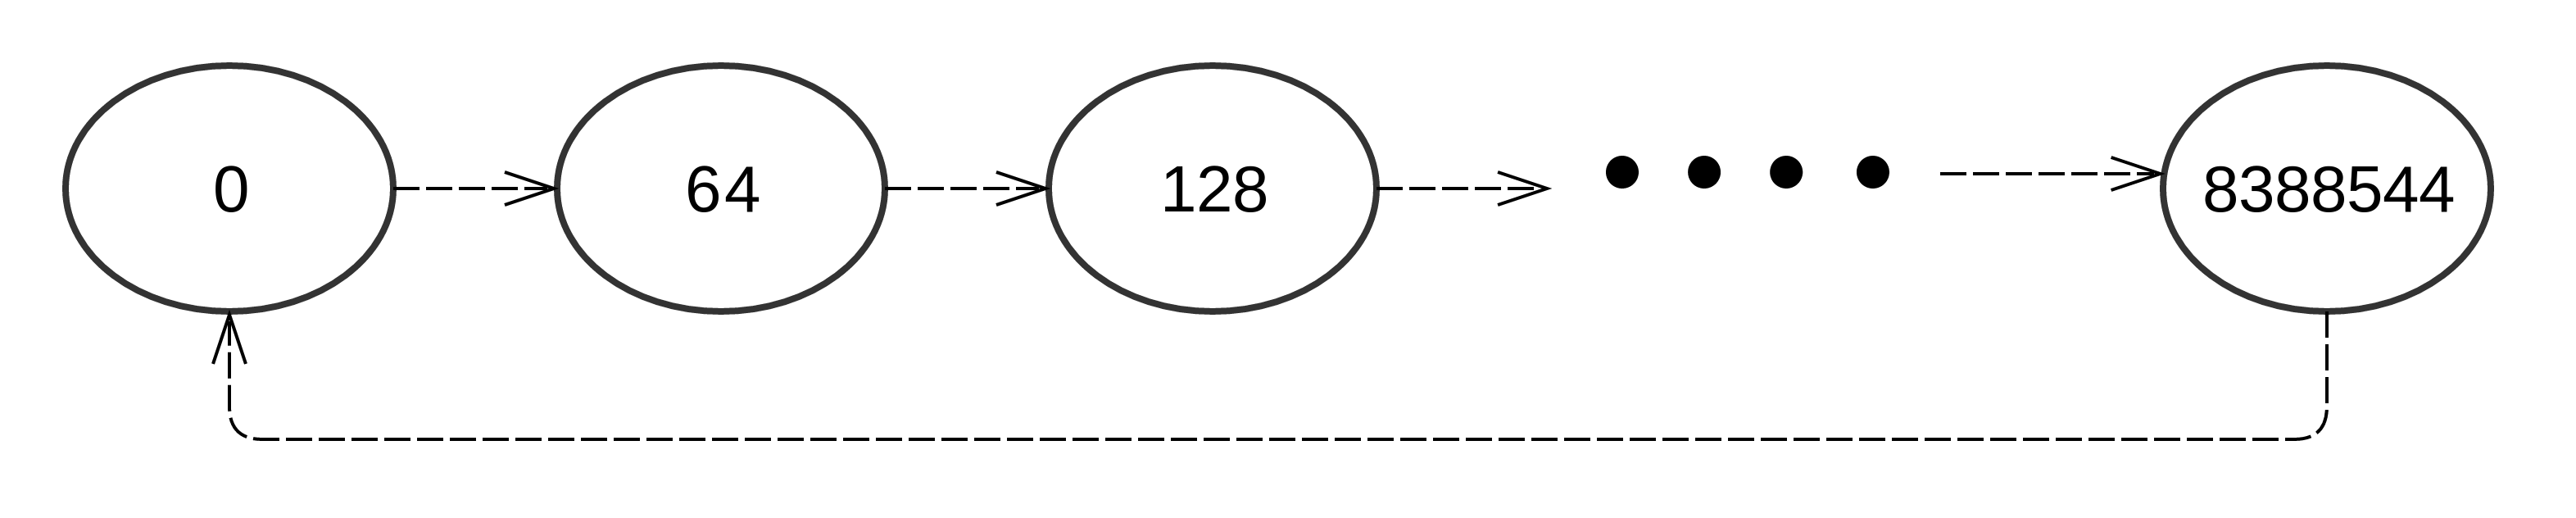
\includegraphics[width=\textwidth]{figures/circularlinkedlist.png}
\caption{Circular Linked List.}
\label{circularlinkedlist}
\end{figure}

The algorithm starts by accessing the buffer as a linked list, thus moving the contents of the buffer into the cache memory and bringing the cache into a known state. Then it measures the access time of a previously fixed variable, which now resides in RAM since the cache is filled with the buffer's contents. The script accesses the variable and measures the time it took to fetch it from RAM. Now the variable is located in the cache memory. The algorithm fetches the variable again and measures the time. The second access should be significantly faster since the variable was fetched from the cache memory.

The script collects multiple measurements by running the algorithm described above and depicted in Listing \ref{orenetal} multiple times. After obtaining the necessary data, the script plots the two sets of measurements as lines. I decided to collect measurements by running the algorithm 100 times. The resulted graph can be seen in Figure \ref{firefox39}.

The role of the website is to collect data by running the algorithm multiple times and plot the two sets. The success of the attack described by Oren et al. \cite{oren2015spy} is measured in how easily it is to distinguish between the two lines. If the graph shows two lines which do not intersect and there is a significant gap between them as in Figure \ref{firefox39} then an adversary could easily distinguish between a cache miss and a cache hit and the system is vulnerable to the cache attack \cite{oren2015spy}. On the other hand, if the graph looks more like Figure \ref{firefox45}, where plotting the time data does not give two non intersecting lines, then the machine is not affected by the aforementioned attack.

\begin{figure}[h]
\centering
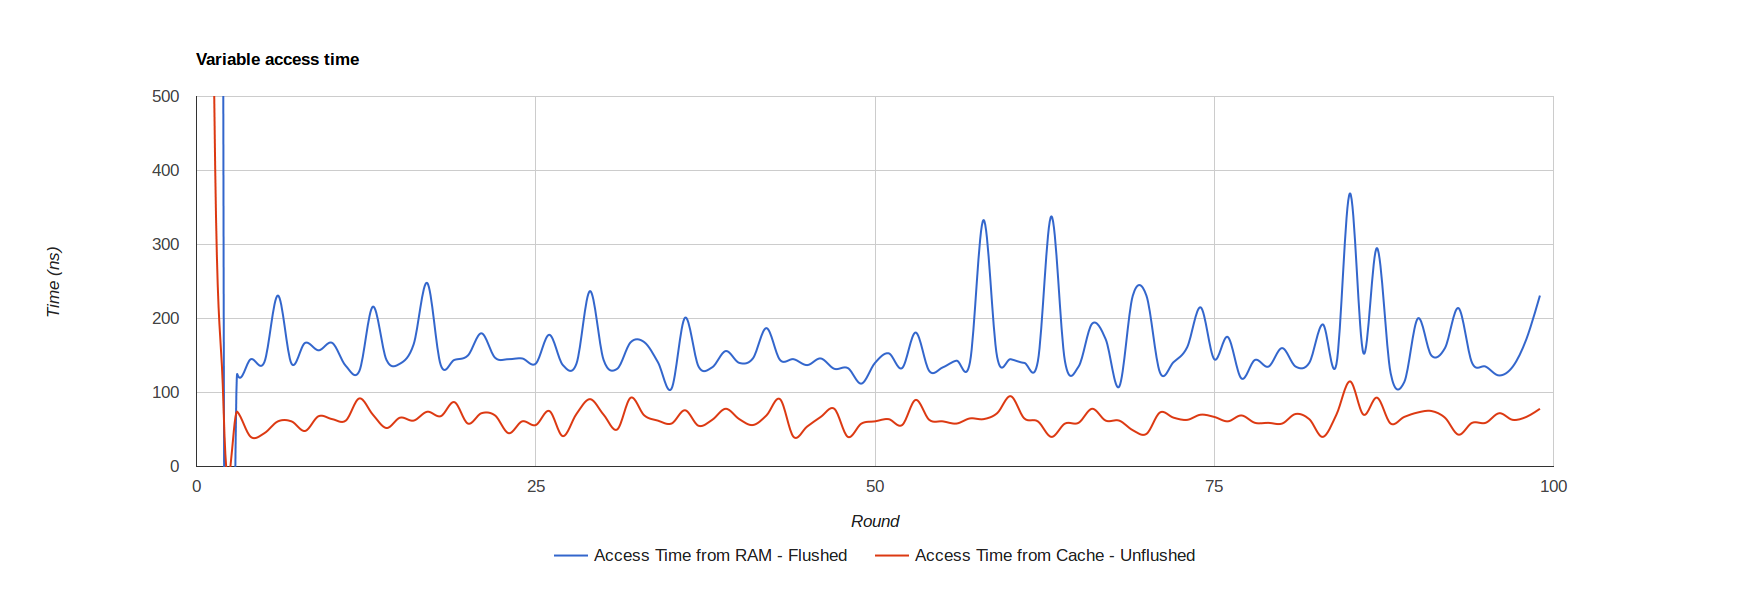
\includegraphics[width=\textwidth]{figures/firefox39.png}
\caption{Variable access times in Firefox 39.}
\label{firefox39}
\end{figure}

\begin{figure}[h]
\centering
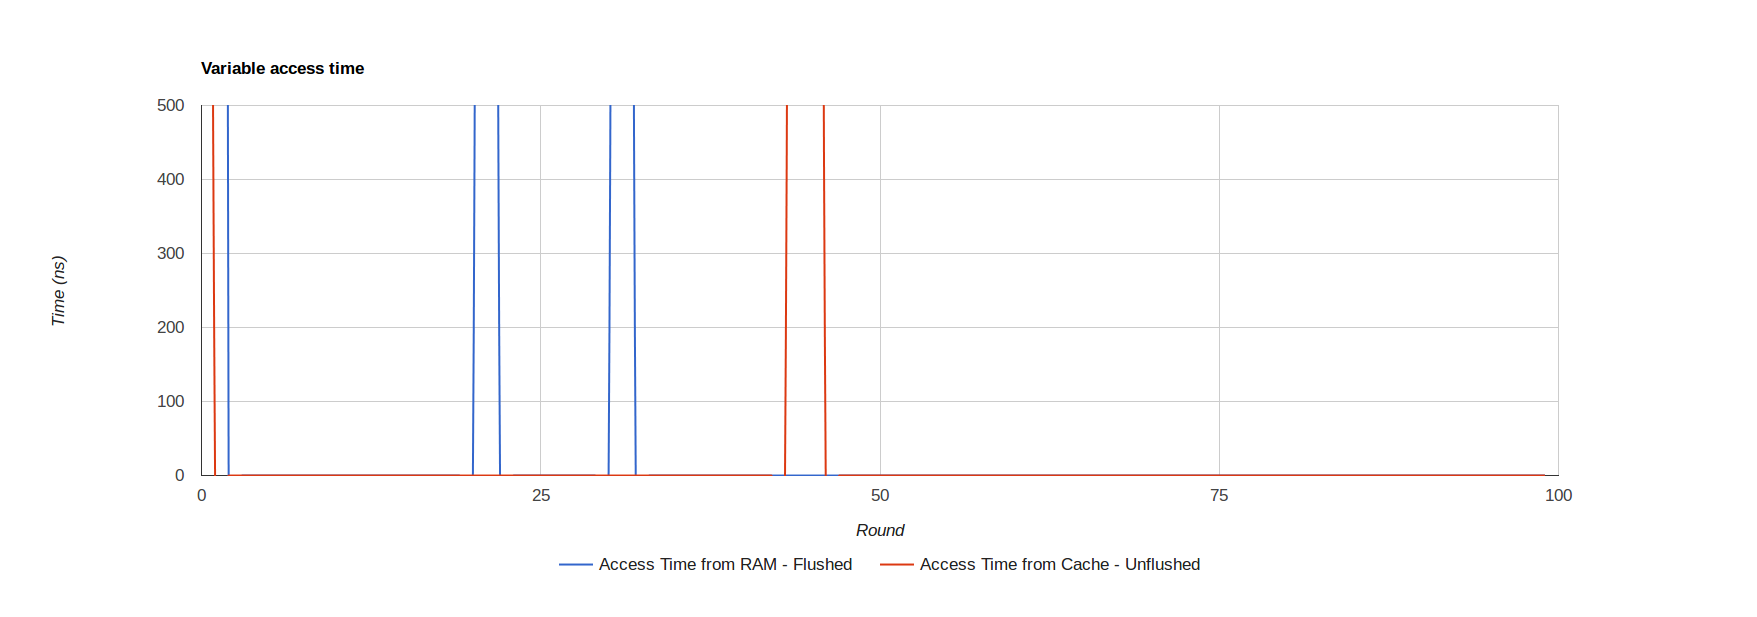
\includegraphics[width=\textwidth]{figures/firefoxnew.png}
\caption{Variable access times in Firefox 45.}
\label{firefox45}
\end{figure}

I discovered that the JavaScript High Resolution Time API has been updated in recent browsers and the measurements are not longer as precise as they used to be. The new version of the timing API provides time measurement accurate to a microsecond. If the difference between the time it takes to access a variable from the cache memory and from RAM is less than one microsecond (100 nanoseconds), an adversary would not be unable to distinguish between the two values. In the attack presented by Oren et al. the difference between the two values is on average under 100 nanoseconds, therefore browsers running the updated version of the API are no longer vulnerable to this attack. 

Figure \ref{firefox39} shows the two distributions, each represented as a line. As it can be seen there is a clear difference in time between a variable accessed from RAM and one accessed from the cache memory. The timing data for Figure \ref{firefox39} was collected using Firefox 39. Figure \ref{firefox45} shows the same attack on the newest version of Firefox, Firefox 45, which contains the recent changes made to the JavaScript High Resolution Time API. The two distributions are indistinguishable, due to the loss in precision of the timing API, the two values are the same in most of the cases.
 
The change in the JavaScript timing API made the attack impossible in JavaScript as there are no known JavaScript APIs which provide the needed functionality. Also, browser vendors are aware of this attack and will not longer provide support for APIs which offer time measurements accurate to less than a microsecond. 

Although the recent changes to the JavaScript High Resolution Time API makes the attack impossible in newer versions of the browser, there are still ways in which the attack can be implemented. Oren et al. decided to use JavaScript because it is the most popular client side language, therefore finding a vulnerability in JavaScript will affect a large number of user; however, there are other client side technologies which might still be affected by a similar attack. 

The attack was possible due to a feature of the JavaScript High Resolution Time API. Although, web applications do not require sub millisecond time measurements, the developers decided to include this feature in the API and browser vendors included the API in their products. Oren et al. were the first who thought about exploiting this feature and discovered that the an attacker could make use of the high precision time measurements provided by the API in order to obtain information about the state of the cache memory. They used this side channel information to compromise users' privacy by disclosing their browsing activity.
 
\section{Van}




%-----------------------------------------------------------------------------

\chapter{Critical Evaluation}
\label{chap:evaluation}


% -----------------------------------------------------------------------------

\chapter{Conclusion}
\label{chap:conclusion}


%%%%%%%%%%%%%%%%%%%%%%%%%%%%%%%%%%%%%%%%%%%%%%%%%%%%%%%%%%%%%%%%%%%%%%%%%%%%%%%%%%%%%%%%
%%%%%%%%%%%%%%%%%%%%%%%%%%%%%%%%%%%%%% The End %%%%%%%%%%%%%%%%%%%%%%%%%%%%%%%%%%%%%%%%%
%%%%%%%%%%%%%%%%%%%%%%%%%%%%%%%%%%%%%%%%%%%%%%%%%%%%%%%%%%%%%%%%%%%%%%%%%%%%%%%%%%%%%%%%

%============================================================================================
% Back Matter

\cleardoublepage
\pagestyle{marked}

\bibliographystyle{ieeetr}
\bibliography{main.bib}

\end{document}